\documentclass[landscape, a4paper]{article}
\usepackage[margin=0cm,top=0.4cm,bottom=0.4cm,left=0.4cm,right=0.4cm]{geometry}
% \usepackage[showframe,margin=0cm,top=0.5cm,bottom=0.5cm,left=0.5cm,right=0.5cm]{geometry}
\usepackage[export]{adjustbox}
\usepackage{ipsum}
\usepackage{xcolor}
\usepackage{caption}
\usepackage{tabularray}
\usepackage{csquotes}
\usepackage{titlesec}
\usepackage{etoolbox} % Add this to your preamble
\usepackage[parfill]{parskip}

\newtoggle{isEnglish}
% \toggletrue{isEnglish}
\togglefalse{isEnglish}

\captionsetup{labelformat=empty, justification=centering, font={color=PrimaryColor}}

\definecolor{PrimaryColor}{HTML}{DD6503}
\definecolor{PrimaryColorDimmed}{HTML}{f1c197}
\colorlet{BoxColor}{gray!10!white}
\newcommand\alert[1]{\textcolor{PrimaryColor}{\textbf{#1}}}

\renewcommand{\labelitemi}{$\textcolor{PrimaryColor}{\bullet}$}
\renewcommand{\labelitemii}{$\textcolor{PrimaryColor}{\blacktriangleright}$}
\renewcommand{\labelitemiii}{$\textcolor{PrimaryColor}{\blacksquare}$}

\renewcommand{\labelenumi}{\textbf{\textcolor{PrimaryColor}{\theenumi.}}}
\renewcommand{\labelenumii}{\textbf{\textcolor{PrimaryColor}{\theenumii.}}}
\renewcommand{\labelenumiii}{\textbf{\textcolor{PrimaryColor}{\theenumiii.}}}

\titleformat{\section}
{\color{PrimaryColor}\normalfont\normalsize\bfseries}
{\thesection}{0.5cm}{}
\titlespacing{\section}{0cm}{0.2cm}{0.2cm}

\titleformat{\subsection}
{\color{PrimaryColor}\normalfont\normalsize\bfseries}
{\thesubsection}{0.5cm}{}
\titlespacing{\subsection}{0cm}{0.1cm}{0.1cm}

\titleformat{\subsubsection}
{\color{PrimaryColor}\normalfont\normalsize\bfseries}
{\thesubsection}{0.5cm}{}
\titlespacing{\subsubsection}{0cm}{0.1cm}{0.1cm}

\begin{document}
\noindent
\centering
\footnotesize
\begin{minipage}[t]{0.31\textwidth}
	\setlength{\parskip}{0.25cm}

	\vspace{0.5cm}

	\textcolor{PrimaryColor}{
		\rule{\linewidth}{0.5mm}
		\vspace{-0.1cm}
		\begin{center}
			\large
			\textsc{California Roll (1 Roll - 8 pieces)}
		\end{center}
		\rule{\linewidth}{0.5mm}
	}

	\subsection*{Ingredients}

	\begin{tblr}{
			cells = {bg=BoxColor},
			row{1} = {PrimaryColor,c,fg=white},
			row{2} = {PrimaryColorDimmed},
			row{8} = {PrimaryColorDimmed},
			row{14} = {PrimaryColorDimmed},
			row{18} = {PrimaryColorDimmed},
			cell{2}{1} = {c=2}{},
			cell{8}{1} = {c=2}{},
			cell{14-21}{1} = {c=2}{},
		}
		\textbf{Ingredient}                               & \textbf{Amount}                        \\
		For the sushi rice:                               &                                        \\
		Sushi rice                                        & 100g                                   \\
		Water                                             & 120ml                                  \\
		Rice vinegar                                      & 15ml                                   \\
		Sugar                                             & 7g                                     \\
		Salt                                              & 2g                                     \\
		For the roll:                                     &                                        \\
		Nori sheet (half sheet):                          & 1 piece ($\sim$18x10 cm)               \\
		Imitation crab stick (surimi):                    & 30 g (2 sticks or shredded equivalent) \\
		Cucumber (seeded):                                & 15 g (cut into matchsticks)            \\
		Ripe avocado:                                     & 20 g (cut into thin strips)            \\
		Toasted white sesame seeds:                       & 1 tsp (3 g)                            \\
		For serving:                                      &                                        \\
		Soy sauce                                         &                                        \\
		Pickled ginger                                    &                                        \\
		Wasabi                                            &                                        \\
		Equipment Needed:                                 &                                        \\
		Bamboo sushi mat (makisu) wrapped in plastic wrap &                                        \\
		Sharp knife (preferably moistened for cutting)    &                                        \\
		Bowl of water (to prevent sticking)               &                                        \\
	\end{tblr}
\end{minipage}%
\hfill%
\vrule width 0.01cm
\hfill%
\begin{minipage}[t]{0.31\textwidth}
	\vspace{0cm}
	\setlength{\parskip}{0.25cm}

	\subsection*{Instructions}
  \vspace{0.25cm}

	\subsubsection*{1. Prepare the Sushi Rice (40–60 mins)}
  \vspace{0.25cm}
	\begin{enumerate}
		\item \alert{Rinse the rice:} Rinse 100 g sushi rice under cold water until the water runs clear. Drain and let rest for 10 minutes.
		\item \alert{Cook the rice:} Combine the rice with 120 ml water in a pot. Bring to a boil, then simmer on low heat for 10 minutes. Let it steam (covered) for an additional 10 minutes.
		\item \alert{Season the rice:} Gently heat 15 ml rice vinegar, 7 g sugar, and 2 g salt until dissolved. Fold into the cooked rice and let cool to body temperature.
	\end{enumerate}

	\subsubsection*{2. Prepare the Fillings (5–10 mins)}
	\begin{itemize}
		\item Peel and seed the cucumber, then slice into thin matchsticks (approx.\ 5 mm wide, 8 cm long).
		\item Cut avocado into thin strips.
		\item Shred or slice imitation crab if necessary.
	\end{itemize}

	\subsubsection*{3. Assemble the Roll (10 mins)}
	\begin{enumerate}
		\item Place plastic-wrapped bamboo mat on a flat surface.
		\item Place half a nori sheet (rough side up) on the mat.
		\item Wet fingers and evenly spread 90–100 g of sushi rice on the nori.
		\item Sprinkle with 3 g sesame seeds.
		\item Carefully flip the nori so rice faces down.
		\item Arrange 30 g imitation crab, 15 g cucumber, and 20 g avocado in a horizontal line, 2–3 cm from the near edge.
		\item Roll the mat forward gently but tightly to form a cylinder.
	\end{enumerate}

	\subsubsection*{4. Cut the Roll (2–3 mins)}
	\begin{itemize}
		\item Dip a sharp knife in water-vinegar mix.
		\item Cut the roll in half, then cut each half into 4 even pieces.
	\end{itemize}

	\subsubsection*{5. Serve}
	\begin{itemize}
		\item Arrange the 8 pieces cut-side up.
		\item Serve with soy sauce, wasabi, and pickled ginger if desired.
	\end{itemize}

	\subsection*{Tips}
	\begin{itemize}
		\item Don’t overload the roll—use thin layers.
		\item Keep hands damp, not wet, when handling rice.
		\item Use plastic wrap over the bamboo mat for easier rolling.
	\end{itemize}

	% 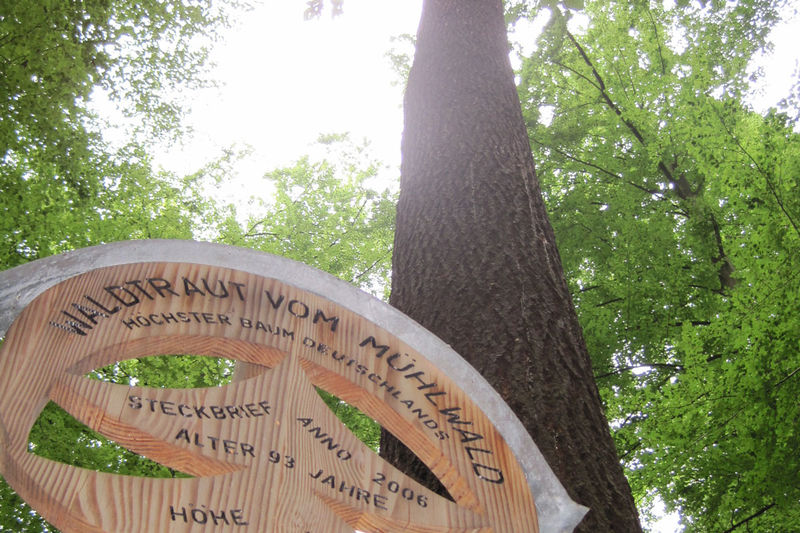
\includegraphics[width=\linewidth]{./figures/waldraud.png}
	%  \captionof{figure}{\iftoggle{isEnglish}{Waldtraut of the Mühlwald, the tallest officially measured tree in Germany}{Waldtraut vom Mühlwald, höchster amtlich vermessener Baum Deutschlands}}
	% \setlength{\parskip}{0.25cm}

\end{minipage}%
\hfill\color{white}%
\vrule width 0.01cm
\hfill\color{black}%
\begin{minipage}[t]{0.31\textwidth}
	\vspace{0cm}
	\setlength{\parskip}{0.25cm}

	asdf

\end{minipage}%

\end{document}
